% mnras_template.tex 
%
% LaTeX template for creating an MNRAS paper
%
% v3.0 released 14 May 2015
% (version numbers match those of mnras.cls)
%
% Copyright (C) Royal Astronomical Society 2015
% Authors:
% Keith T. Smith (Royal Astronomical Society)

% Change log
%
% v3.0 May 2015
%    Renamed to match the new package name
%    Version number matches mnras.cls
%    A few minor tweaks to wording
% v1.0 September 2013
%    Beta testing only - never publicly released
%    First version: a simple (ish) template for creating an MNRAS paper

%%%%%%%%%%%%%%%%%%%%%%%%%%%%%%%%%%%%%%%%%%%%%%%%%%
% Basic setup. Most papers should leave these options alone.
\documentclass[fleqn,usenatbib]{mnras}

% MNRAS is set in Times font. If you don't have this installed (most LaTeX
% installations will be fine) or prefer the old Computer Modern fonts, comment
% out the following line
\usepackage{newtxtext,newtxmath}
% Depending on your LaTeX fonts installation, you might get better results with one of these:
%\usepackage{mathptmx}
%\usepackage{txfonts}

% Use vector fonts, so it zooms properly in on-screen viewing software
% Don't change these lines unless you know what you are doing
\usepackage[T1]{fontenc}

% Allow "Thomas van Noord" and "Simon de Laguarde" and alike to be sorted by "N" and "L" etc. in the bibliography.
% Write the name in the bibliography as "\VAN{Noord}{Van}{van} Noord, Thomas"
\DeclareRobustCommand{\VAN}[3]{#2}
\let\VANthebibliography\thebibliography
\def\thebibliography{\DeclareRobustCommand{\VAN}[3]{##3}\VANthebibliography}


%%%%% AUTHORS - PLACE YOUR OWN PACKAGES HERE %%%%%

% Only include extra packages if you really need them. Common packages are:
\usepackage{graphicx}	% Including figure files
\usepackage{amsmath}	% Advanced maths commands
% \usepackage{amssymb}	% Extra maths symbols

%%%%%%%%%%%%%%%%%%%%%%%%%%%%%%%%%%%%%%%%%%%%%%%%%%

%%%%% AUTHORS - PLACE YOUR OWN COMMANDS HERE %%%%%

% Please keep new commands to a minimum, and use \newcommand not \def to avoid
% overwriting existing commands. Example:
%\newcommand{\pcm}{\,cm$^{-2}$}	% per cm-squared

%%%%%%%%%%%%%%%%%%%%%%%%%%%%%%%%%%%%%%%%%%%%%%%%%%

%%%%%%%%%%%%%%%%%%% TITLE PAGE %%%%%%%%%%%%%%%%%%%

% Title of the paper, and the short title which is used in the headers.
% Keep the title short and informative.
\title{Tidal Features and Remnants in the Milky Way-M31 Merger}

% The list of authors, and the short list which is used in the headers.
% If you need two or more lines of authors, add an extra line using \newauthor
\author[P. G. Shea]{
Peter G. Shea$^{1}$
\\
% List of institutions
$^{1}$Steward Observatory, The University of Arizona, 933 N Cherry Ave, Tucson 85719, US\\
}

% These dates will be filled out by the publisher
% \date{Accepted XXX. Received YYY; in original form ZZZ}

% Enter the current year, for the copyright statements etc.
\pubyear{2025}

% Don't change these lines
\begin{document}
\label{firstpage}
\pagerange{\pageref{firstpage}--\pageref{lastpage}}
\maketitle

% Abstract of the paper
\begin{abstract}
N/A
\end{abstract}

% Select between one and six entries from the list of approved keywords.
% Don't make up new ones.
\begin{keywords}
Tidal Tails -- Tidal Bridges -- Local Group -- Stellar Disk -- Gravitationally Bound
\end{keywords}

%%%%%%%%%%%%%%%%%%%%%%%%%%%%%%%%%%%%%%%%%%%%%%%%%%

%%%%%%%%%%%%%%%%% BODY OF PAPER %%%%%%%%%%%%%%%%%%

\section{Introduction}


Galaxy merging events are the underlying principle of hierarchical galaxy formation theory which proposes accretion of smaller satellites play a significant role galaxy evolution \cite{Wang_Hammer_Athanassoula_Puech_Yang_Flores_2012}. 
These events involve extreme tidal forces which often result in the creation of unique structures within these interacting systems. 
Tidal tails and bridges are streams or spindles of stars and gas or dust which are ejected from their host galaxies throughout the merger process due to gravitational forces exerted on the material. 
They often resemble extended spiral arms which reach out towards (bridge) and away (tail) from the companion satellite \cite{Toomre_Toomre_1972}. 
The study of this form of mass loss and tidal debris provides significant insight into the initial conditions of merging systems, fate of stripped material, and the tidal forces involved in these events.


Studying these tidal remnants of merging events is vital to understand galactic evolution. In particular, these structures can serve as a galactic fossil record of past interactions of galaxies and their satellites past or present \cite{Wang_Hammer_Athanassoula_Puech_Yang_Flores_2012}.  
Based on the shape, prominence, and other physical characteristics of tidal tails and bridges it is possible to determine the strength of tidal forces, pro- and retrograde interactions, and how strongly bound the tail initially was with implications on star formation \cite{Privon_Barnes_Evans_Hibbard_Yun_Mazzarella_Armus_Surace_2013}. 
By studying objects which present these features, it is possible to improve current models of galaxy evolution, structure, and merging events. 


Current research on galaxy mergers has shown the ubiquitous nature of tidal tails and bridges in these systems and has helped to relate physical properties of these structures to characteristics of the merging system. 
The orientation of these tails has been related to disk inclination of the encounters between the two objects and overall orbital geometry of the system \cite{Mihos_2004}. 
Prograde and retrograde encounters also have been shown to created noticeable differences in the strength of the formed tails; prograde encounters create more significant tidal structures compared to retrograde \cite{Privon_Barnes_Evans_Hibbard_Yun_Mazzarella_Armus_Surace_2013}. 
The length and symmetry of these structures created in both interacting galaxies during a merge has also been shown to largely be determined by the speed or severity of the encounter as well as the mass ratio of the objects \cite{Ji_Peirani_Yi_2014,Toomre_Toomre_1972}. 
It been shown that slower encounters tend to create more significant tails and that smaller mass ratios result in more significant tidal features as seen in Fig.~\ref{fig:Ji2014_fig}. 
However, to what extent these remnants can be used to reconstruct all aspects of merging events or identify past events remains open.

\begin{figure}
	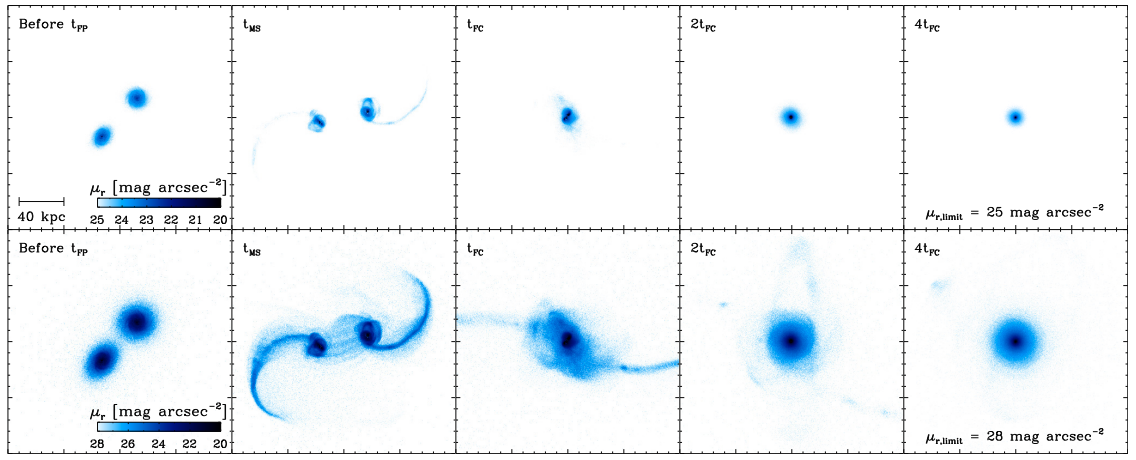
\includegraphics[width=\columnwidth]{Ji2014_fig.png}
    \caption{Mock images of two mass ratio 1:1 mergers taken from \cite{Ji_Peirani_Yi_2014}.}
    \label{fig:Ji2014_fig}
\end{figure}

While many advances have been made in understanding these structures, there are several questions which remain unanswered. 
Perhaps one of the largest is how long these tidal debris exist for and what their fate is as the system evolves. 
The relatively faint nature of these structures has made them difficult to detect and therefore absent in many shallow surveys of galaxy populations. 
Thus, it is unknown whether tidal remnants persist long after the coalescence of merging galaxies or that major mergers which produce these features remain relatively rare. 
Further, it there has been very little exploration as to what becomes of these structures post-coalescence as they are mostly considered to be transient to the merge itself however some research suggest they could seed stellar streams \cite{Wang_Hammer_Athanassoula_Puech_Yang_Flores_2012}. 
Addressing these questions as well as how to better identify these features is vital for furthering models of galaxy evolution.

\section{This Project}

In this investigation we will examine the creation of tidal tails and bridges during the Merger of M31 and the Milky Way. The specific snapshots used in this investigation will be determined by the orbital motion of the centers of mass of the Milky Way and M31 shortly after the periapsis and apoapsis of their orbit. These snapshots include: 275, 280, 285, 335, 340, 345, 410, 420, 425, 430, 435, 470, 475, and 480.
Using this information, it will then be possible to identify disk particles that are within these tidal structures using velocity phase diagrams and track them as the simulation progresses.

Through this investigation, we seek to better understand when in the process of merging these tidal structures are created and in the process identify the fate of this material after the merge has completed. By tracking the identified particles throughout the simulation, it will be possible to determine the lifespan of tidal tails and bridges, as well as if this material remains gravitationally bound to the merge remnant.

Identifying when these structures form, their lifetime, and where this matter eventually ends up will greatly advance our understanding of how galaxies evolve after major merges. This study will help to further increase our understanding of the timeline of tidal structure formation by placing bridge and tail formation events concretely within the simulated merger. Further, by identifying the particles which create these features it is possible to recreate the life of these transient structures to identify lifetime and fate of the matter involved.

\section{Methodology}

The simulation used in this investigation is an N-body simulation of the three major objects of the Local Group -the Milky Way, M31, and M33 - produced by \cite{van_der_Marel_Besla_2012}. In this simulation, gravitational forces between all particles are approximated with the accuracy of this approximation being primarily determined by the distance between the particles. Further, three major components of these galaxies were modeled: the disk, bulge, and dark matter halo. For the galaxies modeled in this simulation, exponential profiles with scale length $R_{d}$ were used for disk profiles, bulge profiles where scaled with $R^{1/4}$, and dark matter halos were modeled using a hernquist profile. Further, M33 was modeled without a bulge due to its insignificant mass.

In order to identify these tidal structures phase diagrams of both the Milky Way and M31 will be created using HiRes data in order to depict the velocity of particles along one axis vs their position in the disk. Clusters of particles which are outliers from the general shape of the phase plot are likely to be tidal tails or bridges and their comprising particles identified as shown in Fig. ~\ref{fig:Phase_box}. The particles which comprise them can then be identified and tracked through later simulations, most notably up to snap 801 which is the end of the simulation as shown in Fig. ~\ref{fig:Tracked_Stars}.

\begin{figure}
	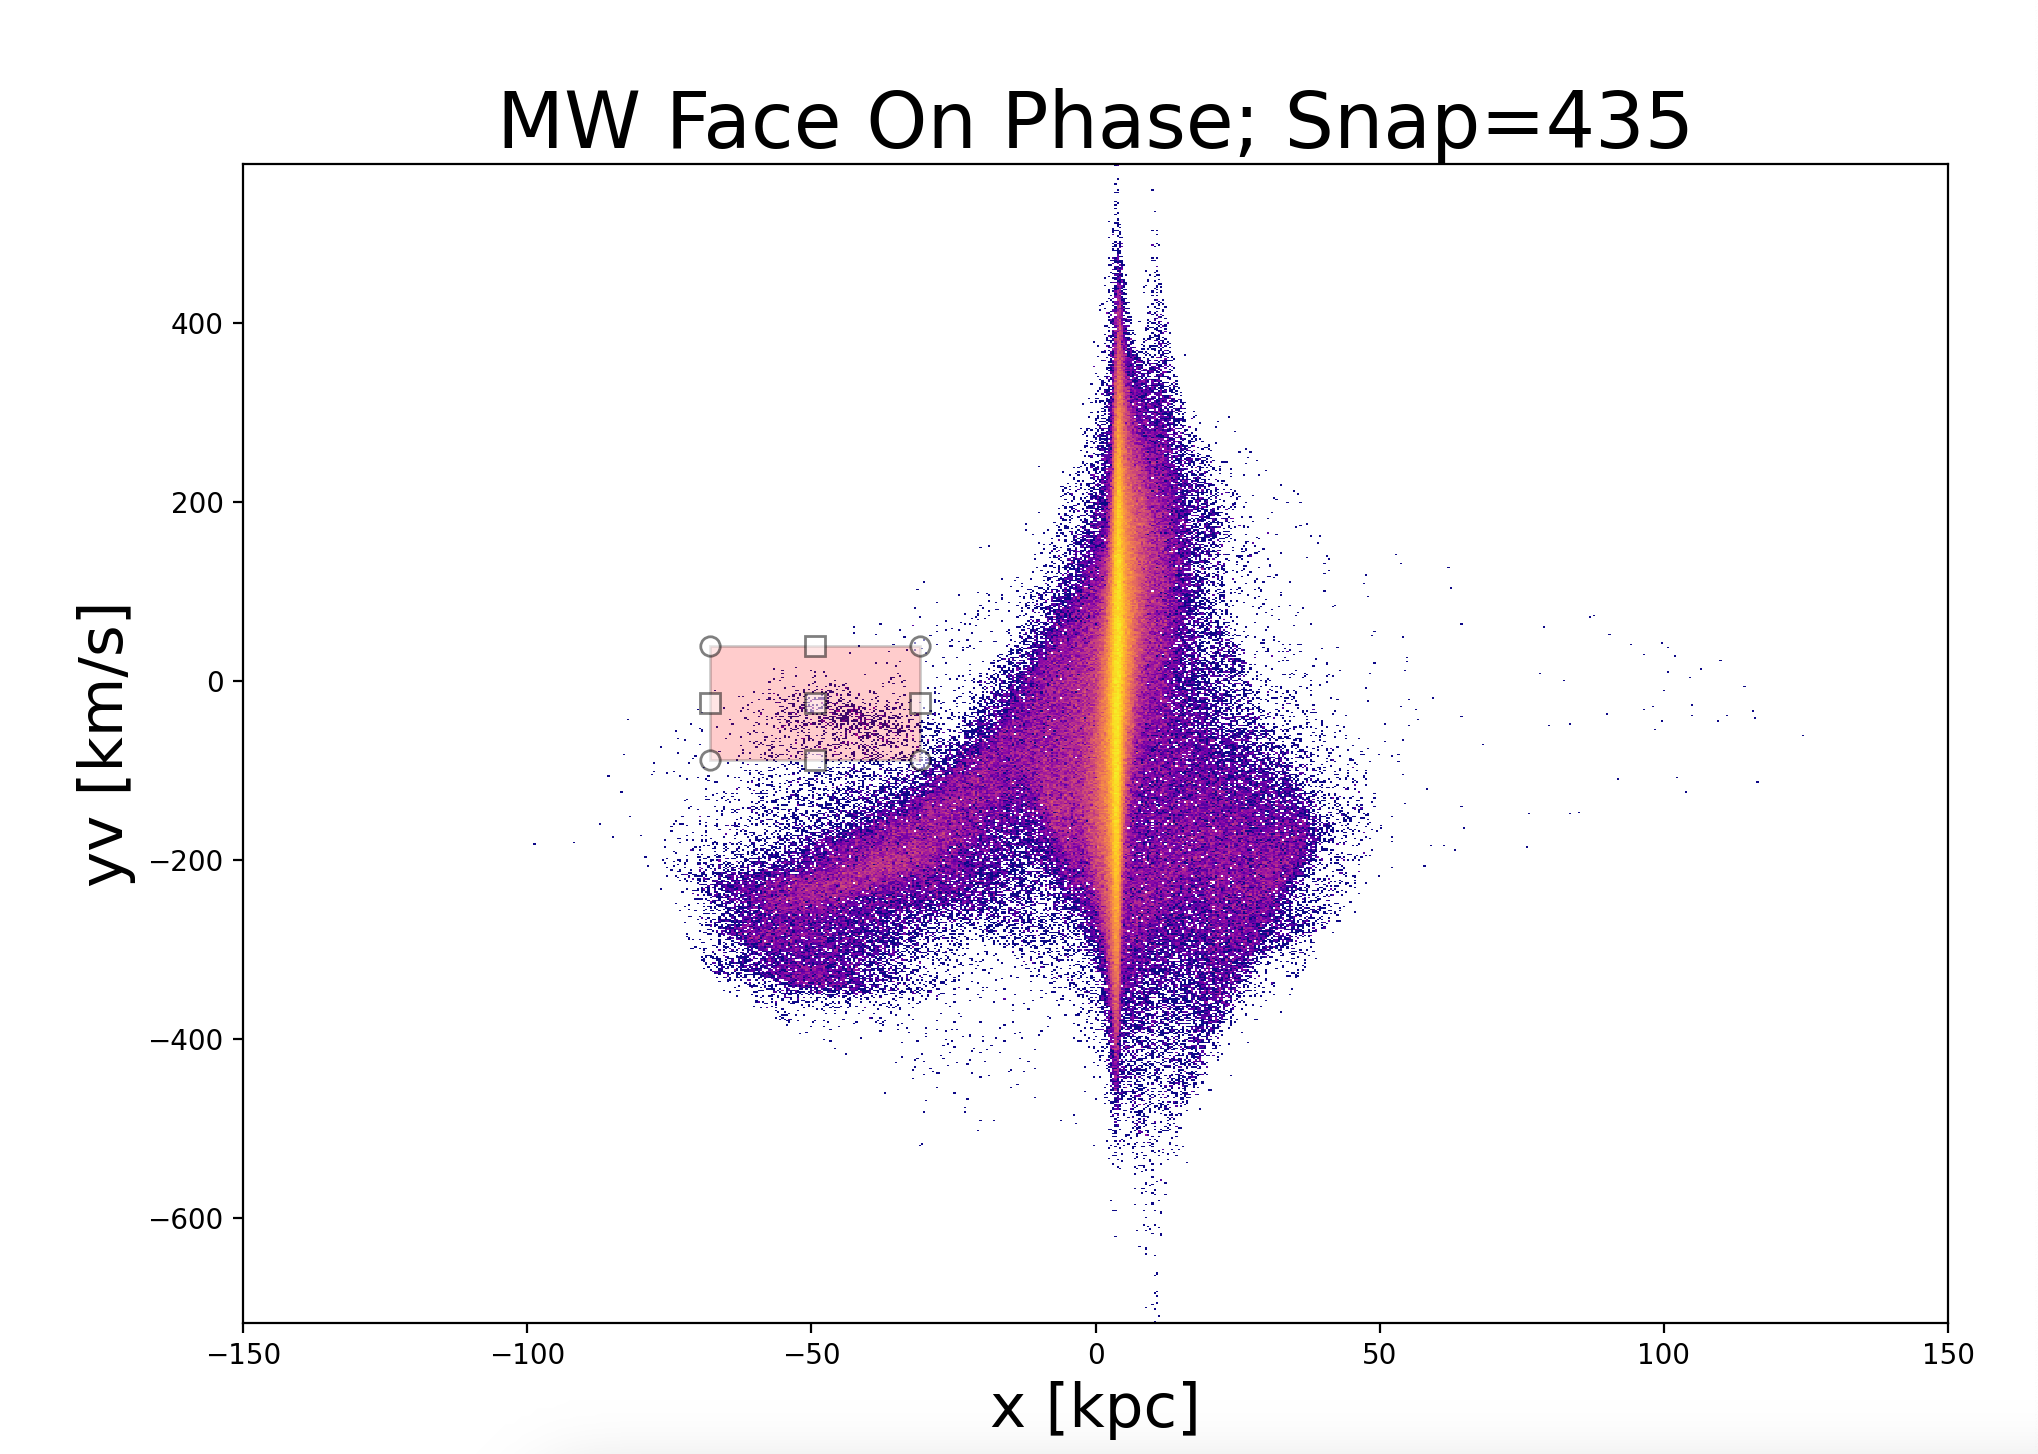
\includegraphics[width=\columnwidth]{Assignment 2/PhaseBox.png}
    \caption{A phase diagram of the Milky Way at snap 435 using HiRes data. The transparent red box is a plotting tool used to identify the index of particles within the specified region.}
    \label{fig:Phase_box}
\end{figure}

\begin{figure}
	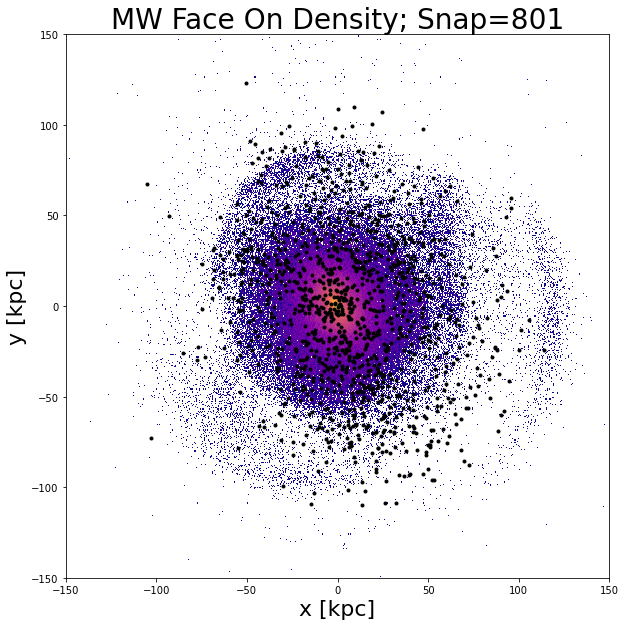
\includegraphics[width=\columnwidth]{Assignment 2/test_tracked_stars.png}
    \caption{A density plot of Milky Way disk particles at snap 100 looking face on to the disk. Black dots in this image are disk particles that were identified to be in the tidal tail or bridge in snap 435.}
    \label{fig:Tracked_Stars}
\end{figure}

 Phase diagrams of both the Milky Way and M31 will be created at snaps 275, 280, 285, 335, 340, 345, 410, 420, 425, 430, 435, 470, 475, and 480. Each plot will be manually analyzed to determine the presence of tidal tails and bridges as shown in Fig. ~\ref{fig:Phase_box}. Disk particles which comprise the identified structures can then be recorded using their indices and tracked through the simulation and ultimately to its conclusion in snap 801 as shown in Fig. ~\ref{fig:Tracked_Stars}. By tracking these stars through the simulation it will be possible to determine the transient lifetime of these tidal structures during the merger process as well as determine where the disk particles which created these structures resided when the simulation ended.

During the Milky Way-M31 merger sequence, tidal tails of various prominence will form at each of the close encounters of the system. 
The most pronounced of these features will persist throughout the length of the simulation. 
Further, while the material will for the most part remain bound to the merger remnant, these tidal structures will potentially remain as seeds for tidal streams as M33 is tidally stripped.

%%%%%%%%%%%%%%%%%%%% REFERENCES %%%%%%%%%%%%%%%%%%

\bibliographystyle{mnras}
\bibliography{ASTR400B} 

% Don't change these lines
\bsp	% typesetting comment
\label{lastpage}
\end{document}

% End of mnras_template.tex
